% TODO checklist:
% - [x] README.md (lines 1-2050): Project structure, architecture diagrams, layer descriptions
% - [x] Q&A.md (Section B, Q8-Q15): Architecture details, system diagrams, cross-cutting concerns
% - [x] src/app.py: FastAPI application structure
% - [x] docker-compose.yml: Container orchestration and service dependencies

\section{Architectural Overview}
\label{sec:arch-overview}

The Cineca Agentic Platform employs a \textbf{three-layer architecture} designed to provide clear separation of concerns, maintainability, and scalability for enterprise AI agent orchestration. This architectural design reflects production requirements gathered from CINECA's operational context, including multi-tenancy, security, observability, and integration with high-performance computing infrastructure.

\subsection{High-Level Architecture}

The platform architecture consists of three primary layers, each with distinct responsibilities:

\begin{enumerate}
    \item \textbf{Presentation Layer}: User-facing interfaces for different personas
    \item \textbf{Core Backend Layer}: Business logic, orchestration, and API services
    \item \textbf{Data and Infrastructure Layer}: Persistence, caching, and external integrations
\end{enumerate}

Figure~\ref{fig:high-level-architecture} illustrates the high-level system architecture with the primary components and their interactions.

\begin{figure}[htbp]
    \centering
    \begin{tikzpicture}[
        node distance=1.5cm,
        layer/.style={rectangle, draw=black, thick, minimum width=12cm, minimum height=1.8cm, align=center},
        component/.style={rectangle, draw=blue!60, fill=blue!10, thick, minimum width=2.5cm, minimum height=1cm, align=center, font=\small},
        db/.style={cylinder, draw=green!60, fill=green!10, thick, minimum width=2cm, minimum height=1cm, aspect=0.3, align=center, font=\small},
        arrow/.style={->, thick, >=stealth}
    ]
        % Presentation Layer
        \node[layer, fill=orange!10] (pres) at (0, 4) {};
        \node[above] at (0, 5.1) {\textbf{Presentation Layer}};
        \node[component] (chat) at (-3, 4) {Next.js\\Agent Chat UI};
        \node[component] (panel) at (0, 4) {Streamlit\\Control Panel};
        \node[component] (api) at (3, 4) {REST API\\Clients};
        
        % Core Backend Layer
        \node[layer, fill=blue!10] (core) at (0, 1.5) {};
        \node[above] at (0, 2.6) {\textbf{Core Backend Layer}};
        \node[component] (fastapi) at (-3.5, 1.5) {FastAPI\\App};
        \node[component] (orch) at (-0.5, 1.5) {Orchestrator\\Service};
        \node[component] (mcp) at (2.5, 1.5) {MCP Tools\\(34 tools)};
        
        % Data Layer
        \node[layer, fill=green!10] (data) at (0, -1.5) {};
        \node[above] at (0, -0.4) {\textbf{Data \& Infrastructure Layer}};
        \node[db] (pg) at (-4, -1.5) {PostgreSQL};
        \node[db] (redis) at (-1, -1.5) {Redis};
        \node[db] (mg) at (2, -1.5) {Memgraph};
        \node[component] (llm) at (4.5, -1.5) {LLM\\Providers};
        
        % Arrows
        \draw[arrow] (chat) -- (fastapi);
        \draw[arrow] (panel) -- (fastapi);
        \draw[arrow] (api) -- (fastapi);
        \draw[arrow] (fastapi) -- (orch);
        \draw[arrow] (orch) -- (mcp);
        \draw[arrow] (orch) -- (pg);
        \draw[arrow] (orch) -- (redis);
        \draw[arrow] (mcp) -- (mg);
        \draw[arrow] (orch) -- (llm);
    \end{tikzpicture}
    \caption{High-level architecture of the Cineca Agentic Platform showing the three-layer design with primary components.}
    \label{fig:high-level-architecture}
\end{figure}

\subsection{Three-Layer Design Rationale}

The three-layer architecture was selected based on several enterprise requirements and design principles:

\paragraph{Separation of Concerns}
Each layer has a single, well-defined responsibility. The Presentation Layer handles user interaction and visualization; the Core Backend Layer encapsulates business logic, agent orchestration, and security enforcement; the Data Layer manages persistence and external system integration. This separation enables independent development, testing, and scaling of each layer.

\paragraph{Horizontal Scalability}
The stateless design of the Core Backend Layer allows horizontal scaling through container replication. Session state and job queues are externalized to Redis, enabling multiple FastAPI instances to share workload while maintaining consistency.

\paragraph{Technology Flexibility}
The adapter pattern employed in the Data Layer abstracts external dependencies (LLM providers, databases) behind consistent interfaces. This design enables swapping implementations without affecting business logic---for example, switching between OpenAI and Ollama providers, or migrating between graph database vendors.

\paragraph{Observability by Design}
Cross-cutting concerns (logging, metrics, tracing) are implemented as middleware and decorators that wrap all layer boundaries. This ensures consistent observability across the entire request lifecycle without polluting business logic.

\subsection{Component Inventory}

Table~\ref{tab:component-inventory} provides a quantitative overview of the platform's major components, reflecting the scale and complexity of the implementation.

\begin{table}[htbp]
    \centering
    \caption{Quantitative inventory of major platform components.}
    \label{tab:component-inventory}
    \begin{tabular}{llr}
        \toprule
        \textbf{Category} & \textbf{Component} & \textbf{Count/Size} \\
        \midrule
        API Layer & Endpoint count & 76 \\
        API Layer & Router modules & 23 \\
        API Layer & Schema definitions & 200+ \\
        \midrule
        Services & Orchestrator (lines) & 8,263 \\
        Services & Background tasks & 4 \\
        Services & Health probes & 6 \\
        \midrule
        MCP Tools & Tool categories & 17 \\
        MCP Tools & Total tools & 34 \\
        \midrule
        Data Layer & PostgreSQL tables & 15+ \\
        Data Layer & Alembic migrations & 26 \\
        Data Layer & Redis key patterns & 10+ \\
        Data Layer & Memgraph node types & 14 \\
        \midrule
        Testing & Test files & 272 \\
        Testing & Test lines & $\sim$64,500 \\
        \midrule
        Total & Python source lines & $\sim$77,000 \\
        \bottomrule
    \end{tabular}
\end{table}

\subsection{Deployment Topology}

The platform is designed for containerized deployment using Docker Compose for development and Kubernetes for production. The deployment topology includes:

\begin{itemize}
    \item \textbf{Application containers}: FastAPI backend (1--N replicas), background workers
    \item \textbf{Database containers}: PostgreSQL (primary + optional replica), Redis (standalone or Sentinel), Memgraph
    \item \textbf{Observability stack}: Prometheus, Grafana, optional OpenTelemetry Collector
    \item \textbf{Reverse proxy}: Nginx for TLS termination, rate limiting, and load balancing
    \item \textbf{UI containers}: Next.js (static or SSR), Streamlit
\end{itemize}

Figure~\ref{fig:deployment-topology} illustrates the container orchestration and network topology for a production deployment.

\begin{figure}[htbp]
    \centering
    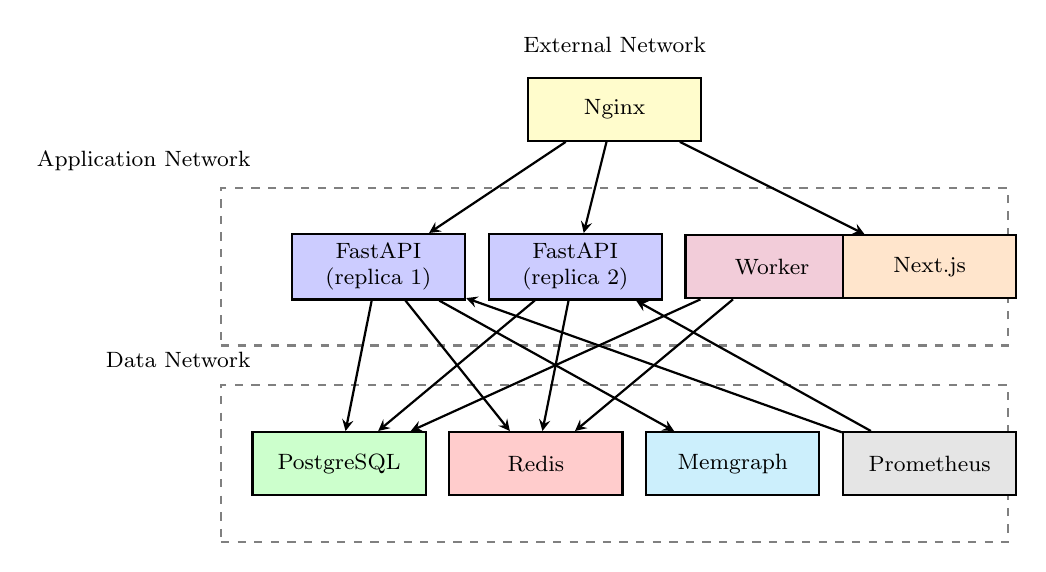
\begin{tikzpicture}[
        node distance=1.2cm,
        container/.style={rectangle, draw=black, thick, minimum width=2.2cm, minimum height=0.8cm, align=center, font=\footnotesize},
        network/.style={rectangle, draw=gray, dashed, thick, minimum width=10cm, minimum height=2cm},
        arrow/.style={->, thick, >=stealth}
    ]
        % External
        \node[container, fill=yellow!20] (nginx) at (0, 3) {Nginx};
        \node[above] at (0, 3.6) {\footnotesize External Network};
        
        % Application Network
        \node[network] (appnet) at (0, 1) {};
        \node[above left] at (-4.5, 2.1) {\footnotesize Application Network};
        \node[container, fill=blue!20] (api1) at (-3, 1) {FastAPI\\(replica 1)};
        \node[container, fill=blue!20] (api2) at (-0.5, 1) {FastAPI\\(replica 2)};
        \node[container, fill=purple!20] (worker) at (2, 1) {Worker};
        \node[container, fill=orange!20] (ui) at (4, 1) {Next.js};
        
        % Data Network
        \node[network] (datanet) at (0, -1.5) {};
        \node[above left] at (-4.5, -0.4) {\footnotesize Data Network};
        \node[container, fill=green!20] (pg) at (-3.5, -1.5) {PostgreSQL};
        \node[container, fill=red!20] (redis) at (-1, -1.5) {Redis};
        \node[container, fill=cyan!20] (mg) at (1.5, -1.5) {Memgraph};
        \node[container, fill=gray!20] (prom) at (4, -1.5) {Prometheus};
        
        % Arrows
        \draw[arrow] (nginx) -- (api1);
        \draw[arrow] (nginx) -- (api2);
        \draw[arrow] (nginx) -- (ui);
        \draw[arrow] (api1) -- (pg);
        \draw[arrow] (api1) -- (redis);
        \draw[arrow] (api2) -- (pg);
        \draw[arrow] (api2) -- (redis);
        \draw[arrow] (worker) -- (redis);
        \draw[arrow] (worker) -- (pg);
        \draw[arrow] (api1) -- (mg);
        \draw[arrow] (prom) -- (api1);
        \draw[arrow] (prom) -- (api2);
    \end{tikzpicture}
    \caption{Production deployment topology showing container orchestration across network segments.}
    \label{fig:deployment-topology}
\end{figure}

\subsection{Cross-Cutting Concerns Overview}

The platform implements fourteen cross-cutting concerns that span all architectural layers. These concerns are enforced through middleware, decorators, and shared utilities rather than being embedded in business logic. Table~\ref{tab:cross-cutting-summary} summarizes these concerns; detailed implementations are discussed in Section~\ref{sec:core-backend}.

\begin{table}[htbp]
    \centering
    \caption{Summary of cross-cutting concerns implemented across all layers.}
    \label{tab:cross-cutting-summary}
    \small
    \begin{tabular}{lll}
        \toprule
        \textbf{Concern} & \textbf{Implementation} & \textbf{Layer(s)} \\
        \midrule
        Logging & Structlog with JSON/console output & All \\
        Metrics & Prometheus counters, histograms, gauges & All \\
        Tracing & OpenTelemetry spans & All \\
        Security & JWT validation, RBAC, tenant isolation & Core, Data \\
        Rate Limiting & Sliding window (Redis-backed) & Core \\
        PII Scrubbing & Detection and redaction & Core \\
        Error Handling & RFC 7807 Problem Details & Core \\
        Pagination & Cursor-based, stateless & Core \\
        ETags/Caching & Conditional requests & Core \\
        Idempotency & Redis-backed keys & Core \\
        Deprecation & Headers and version tracking & Core \\
        Request ID & Trace-request correlation & All \\
        Circuit Breakers & Resilience for external calls & Data \\
        Health Probes & Kubernetes liveness/readiness & Core \\
        \bottomrule
    \end{tabular}
\end{table}

\subsection{Request Flow}

A typical request through the platform follows this path:

\begin{enumerate}
    \item \textbf{Ingress}: Request arrives at Nginx, which terminates TLS and performs initial rate limiting.
    \item \textbf{Middleware}: FastAPI middleware extracts request ID, validates JWT, resolves tenant context, and binds logging context.
    \item \textbf{Router}: The appropriate router handler is invoked based on URL path and HTTP method.
    \item \textbf{Service}: Business logic is executed in the service layer, potentially invoking the orchestrator for agent runs.
    \item \textbf{Persistence}: Data is read from or written to PostgreSQL (authoritative state), with Redis providing caching and queuing.
    \item \textbf{Response}: Results are serialized through Pydantic schemas, response headers are added (ETag, X-Request-ID), and metrics are recorded.
\end{enumerate}

This layered flow ensures consistent application of security policies, observability instrumentation, and error handling regardless of the specific endpoint being accessed.
